\documentclass[10pt]{article}
\usepackage[polish]{babel}
\usepackage[utf8]{inputenc}
\usepackage[T1]{fontenc}
\usepackage{amsmath}
\usepackage{amsfonts}
\usepackage{amssymb}
\usepackage[version=4]{mhchem}
\usepackage{stmaryrd}
\usepackage{graphicx}
\usepackage[export]{adjustbox}
\graphicspath{ {./images/} }
\usepackage{fvextra, csquotes}

\title{EGZAMIN MATURALNY W ROKU SZKOLNYM 2015/2016 }

\author{MATEMATYKA POZIOM ROZSZERZONY}
\date{}


%New command to display footnote whose markers will always be hidden
\let\svthefootnote\thefootnote
\newcommand\blfootnotetext[1]{%
  \let\thefootnote\relax\footnote{#1}%
  \addtocounter{footnote}{-1}%
  \let\thefootnote\svthefootnote%
}

%Overriding the \footnotetext command to hide the marker if its value is `0`
\let\svfootnotetext\footnotetext
\renewcommand\footnotetext[2][?]{%
  \if\relax#1\relax%
    \ifnum\value{footnote}=0\blfootnotetext{#2}\else\svfootnotetext{#2}\fi%
  \else%
    \if?#1\ifnum\value{footnote}=0\blfootnotetext{#2}\else\svfootnotetext{#2}\fi%
    \else\svfootnotetext[#1]{#2}\fi%
  \fi
}

\newcommand\Varangle{\mathop{{<\!\!\!\!\!\text{\small)}}\:}\nolimits}

\begin{document}
\maketitle
FORMUŁA OD 2015\\
(,NOWA MATURA")

ZASADY OCENIANIA ROZWIĄZAŃ ZADAŃ\\
ARKUSZ MMA-P1

\section*{Ogólne zasady oceniania}
Uwaga: Akceptowane sq wszystkie odpowiedzi merytorycznie poprawne i spetniajace warunki zadania.

Zadanie 1. (0-1)

\begin{center}
\begin{tabular}{|l|l|c|}
\hline
\multicolumn{1}{|c|}{Wymagania ogólne} & \multicolumn{1}{|c|}{Wymagania szczególowe} & \begin{tabular}{c}
Poprawna \\
odp. (1 p.) \\
\end{tabular} \\
\hline
\begin{tabular}{l}
II. Wykorzystanie \\
i interpretowanie \\
reprezentacji. \\
\end{tabular} & \begin{tabular}{l}
2. Wyrażenia algebraiczne. Zdajacy używa wzorów \\
skróconego mnożenia na $(a \pm b)^{3}$ oraz $a^{3} \pm b^{3}$ \\
(R2.1). \\
\end{tabular} & C \\
\hline
\end{tabular}
\end{center}

\section*{Zadanie 2. (0-1)}
\begin{center}
\begin{tabular}{|l|l|c|}
\hline
\begin{tabular}{l}
I. Wykorzystanie \\
i tworzenie informacji. \\
\end{tabular} & \begin{tabular}{l}
3. Równania i nierówności. Zdający stosuje \\
twierdzenie o reszcie $z$ dzielenia wielomianu przez \\
dwumian $x-a(R 3.4)$. \\
\end{tabular} & D \\
\hline
\end{tabular}
\end{center}

\section*{Zadanie 3. (0-1)}
II. Wykorzystanie i interpretowanie reprezentacji.\\
4. Funkcje. Zdający na podstawie wykresu funkcji\\
$y=f(x)$ szkicuje wykresy funkcji $y=|f(x)|, y=c \cdot f(x)$, $y=f(c x)$ (R4.1).

B

\section*{Zadanie 4. (0-1)}
\begin{center}
\begin{tabular}{|l|l|l|}
\hline
\begin{tabular}{l}
II. Wykorzystanie \\
i interpretowanie \\
reprezentacji. \\
\end{tabular} & \begin{tabular}{l}
11. Rachunek różniczkowy. Zdający oblicza \\
pochodne funkcji wymiernych (R11.2). \\
\end{tabular} & A \\
\hline
\end{tabular}
\end{center}

Zadanie 5. (0-1)

\begin{center}
\begin{tabular}{|l|l|l|}
\hline
\begin{tabular}{l}
II. Wykorzystanie \\
i interpretowanie \\
reprezentacji. \\
\end{tabular} & \begin{tabular}{l}
11. Rachunek różniczkowy. Zdający oblicza granice \\
funkcji (i granice jednostronne), korzystając \\
z twierdzeń o działaniach na granicach i z własności \\
funkcji ciągłych (R11.1). \\
\end{tabular} & D \\
\hline
\end{tabular}
\end{center}

Zadanie 6. (0-2)\\
III. Modelowanie matematyczne.\\
10. Elementy statystyki opisowej. Teoria prawdopodobieństwa i kombinatoryka. Zdający 753 oblicza prawdopodobieństwo warunkowe (R10.2).\\
III. Modelowanie matematyczne.\\
5. Ciągi. Zdający rozpoznaje szeregi geometryczne zbieżne i oblicza ich sumy (R5.3).

\section*{Przykładowe rozwiązania}
\section*{I sposób}
Pierwszym wyrazem ciągu $\left(a_{n}\right)$ jest $a_{1}=\frac{1}{2 x-371}$. Ilorazem tego ciągu jest $q=\frac{1}{2 x-371}$.\\
Ponieważ wszystkie wyrazy tego ciągu są dodatnie, więc szereg jest zbieżny, gdy $0<\frac{1}{2 x-371}<1$. Zatem

$$
2 x-371>0 \text { i } 2 x-371>1
$$

Stąd

$$
\begin{aligned}
2 x & >372, \\
x & >186 .
\end{aligned}
$$

Zatem szukaną liczbą całkowitą jest 187.

\section*{II sposób}
Pierwszym wyrazem ciągu $\left(a_{n}\right)$ jest $a_{1}=\frac{1}{2 x-371}$, ilorazem tego ciągu zaś jest $q=\frac{1}{2 x-371}$. Szereg geometryczny jest zbieżny wtedy i tylko wtedy, gdy: $\left|\frac{1}{2 x-371}\right|<1$.

Rozwiązujemy powyższą nierówność:

$$
\begin{gathered}
-1<\frac{1}{2 x-371}<1, \\
0<\frac{2 x-370}{2 x-371} \wedge \frac{-2 x+372}{2 x-371}<0, \\
x \neq 185,5 \wedge(x-185)(x-185,5)>0 \wedge(x-186)(x-185,5)>0, \\
x \in(-\infty, 185) \cup(186,+\infty) .
\end{gathered}
$$

Wszystkie wyrazy ciągu $\left(a_{n}\right)$ są dodatnie, więc $x \in(186,+\infty)$. Zatem szukaną liczbą całkowitą jest 187.

\section*{Schemat punktowania}
Zdający otrzymuje\\
gdy zapisze $q=\frac{1}{2 x-371}$ i na tym poprzestanie lub dalej popełnia błędy.\\
Zdający otrzymuje 2 p.\\
gdy zapisze najmniejszą liczbę całkowitą $x$, dla której nieskończony szereg jest zbieżny, tzn. liczbę 187, o ile wynik nie został uzyskany w wyniku błędnego rozwiązania.

\section*{Uwaga:}
Jeżeli zdający bez stosownych obliczeń i bez komentarza zapisuje, że szukaną liczbą jest 187 i na tym zakończy, to otrzymuje 1 punkt.

Zadanie 8. (0-3)\\
V. Rozumowanie i argumentacja.\\
2. Wyrażenia algebraiczne. Zdający używa wzorów skróconego mnożenia na $(a \pm b)^{2}$ oraz $a^{2}-b^{2}$ (2.1).

\section*{Przykładowe rozwiązanie}
I sposób\\
Dla dowolnych liczb dodatnich $x$ i $y$ takich, że $x^{2}+y^{2}=2$ nierówność $x+y \leq 2$ jest równoważna kolejno nierównościom

$$
\begin{gathered}
(x+y)^{2} \leq 4, \\
x^{2}+2 x y+y^{2} \leq 4, \\
x^{2}+2 x y+y^{2} \leq 2 \cdot 2, \\
x^{2}+y^{2}+2 x y \leq 2\left(x^{2}+y^{2}\right), \\
x^{2}+y^{2}+2 x y \leq 2 x^{2}+2 y^{2}, \\
x^{2}+y^{2}-2 x y \geq 0, \\
(x-y)^{2} \geq 0 .
\end{gathered}
$$

Ta ostatnia nierówność jest prawdziwa dla dowolnych liczb rzeczywistych $x$ i $y$. To kończy dowód.

\section*{Schemat punktowania I sposobu rozwiązania}
Zdający otrzymuje 1 p.\\
gdy uzasadni, że dla dowolnych liczb dodatnich $x$ i $y$ takich, że $x^{2}+y^{2}=2$ nierówność $x+y \leq 2$ jest równoważna nierówności $x^{2}+2 x y+y^{2} \leq 2 \cdot 2$ i na tym poprzestanie lub dalej popełnia błędy.\\
Zdający otrzymuje 2 p. gdy uzasadni, że dla dowolnych liczb dodatnich $x$ i $y$ takich, że $x^{2}+y^{2}=2$ nierówność $x+y \leq 2$ jest równoważna nierówności $x^{2}+y^{2}+2 x y \leq 2\left(x^{2}+y^{2}\right)$ i na tym poprzestanie lub dalej popełnia błędy.

\footnotetext{Zdający otrzymuje 3 p. gdy przeprowadzi pełne rozumowanie.
}\section*{Przykładowe rozwiązanie}
\section*{II sposób}
Niech $x$ i $y$ będą dowolnymi dodatnimi liczbami rzeczywistymi takimi, że $x^{2}+y^{2}=2$.\\
Obie strony nierówności $x+y \leq 2$ są dodatnie, więc podnosząc obie strony nierówności do kwadratu otrzymujmy nierówność równoważną

$$
x^{2}+y^{2}+2 x y \leq 4 .
$$

Stąd otrzymujemy $2+2 x y \leq 4$, więc $x y \leq 1$.\\
Obie strony tej nierówności $x y \leq 1$ są dodatnie, więc podnosząc obie strony nierówności do kwadratu otrzymujmy nierówność równoważną

$$
x^{2} y^{2} \leq 1 .
$$

Z założenia $y^{2}=2-x^{2}$. Wówczas nierówność $x^{2} y^{2} \leq 1$ jest równoważna nierównościom

$$
\begin{gathered}
x^{2}\left(2-x^{2}\right) \leq 1 \\
-x^{4}+2 x^{2} \leq 1 \\
x^{4}-2 x^{2}+1 \geq 0 \\
\left(x^{2}-1\right)^{2} \geq 0
\end{gathered}
$$

Ta ostatnia nierówność jest prawdziwa dla każdej liczby rzeczywistej $x$. To kończy dowód.

\section*{Schemat punktowania II sposobu rozwiązania Zdający otrzymuje}
gdy uzasadni, że dla dowolnych liczb dodatnich $x$ i $y$ takich, że $x^{2}+y^{2}=2$ nierówność $x+y \leq 2$ jest równoważna nierówności $x y \leq 1$ i na tym poprzestanie lub dalej popełnia błędy.\\
Zdający otrzymuje\\
gdy zapisze nierówność z jedną niewiadomą, np. $x\left(\sqrt{2-x^{2}}\right) \leq 1$ i na tym poprzestanie lub dalej popełnia błędy.

\section*{Zdający otrzymuje}
gdy przeprowadzi pełne rozumowanie.

\section*{Przykładowe rozwiązanie}
\section*{III sposób}
Niech $x$ i $y$ będą dowolnymi dodatnimi liczbami rzeczywistymi takimi, że $x^{2}+y^{2}=2$. Wykorzystując nierówność między średnią arytmetyczną i średnią kwadratową, otrzymujemy

$$
\frac{x+y}{2} \leq \sqrt{\frac{x^{2}+y^{2}}{2}}
$$

Stąd i z równości $x^{2}+y^{2}=2$ wynika, że $\frac{x+y}{2} \leq \sqrt{\frac{2}{2}}=1$, czyli $x+y \leq 2$. To kończy dowód.

\section*{Schemat punktowania III sposobu rozwiązania}
\section*{Zdający otrzymuje}
gdy zapisze nierówność między średnią arytmetyczną i średnią kwadratową

$$
\frac{x+y}{2} \leq \sqrt{\frac{x^{2}+y^{2}}{2}}
$$

i na tym poprzestanie lub dalej popełnia błędy.\\
Zdający otrzymuje 3 p.\\
gdy zapisze nierówność między średnią arytmetyczną i średnią kwadratową i na tej podstawie uzasadni prawdziwość nierówności $x+y \leq 2$.

\section*{Przykładowe rozwiązanie}
\section*{IV sposób}
Dla dowolnych liczb dodatnich $x$ i $y$ takich, że $x^{2}+y^{2}=2$ nierówność $x+y \leq 2$ jest równoważna kolejno nierównościom

$$
\begin{gathered}
(x+y)^{2} \leq 4, \\
x^{2}+2 x y+y^{2} \leq 4, \\
2+2 x y \leq 4, \\
x y \leq 1 \\
x^{2} y^{2} \leq 1
\end{gathered}
$$

Możemy przyjąć, że $x^{2}=1-p$ oraz $y^{2}=1+p$, gdzie $-1<p<1$. Zatem nierówność $x^{2} y^{2} \leq 1$ przyjmuje postać $(1-p)(1+p) \leq 1$, czyli $1-p^{2} \leq 1$, co jest prawdą dla każdej liczby rzeczywistej $p$, więc, w szczególności, dla każdej liczby $-1<p<1$. To kończy dowód.

\section*{Schemat punktowania IV sposobu rozwiązania}
Zdający otrzymuje 1 p.\\
gdy uzasadni, że dla dowolnych liczb dodatnich $x$ i $y$ takich, że $x^{2}+y^{2}=2$ nierówność $x+y \leq 2$ jest równoważna nierówności $x y \leq 1$ i na tym poprzestanie lub dalej popełnia błędy.

Zdający otrzymuje 2 p. gdy uzasadni, że dla dowolnych liczb dodatnich $x$ i $y$ takich, że $x^{2}+y^{2}=2$ nierówność $x+y \leq 2$ jest równoważna nierówności $x^{2} y^{2} \leq 1$ oraz przyjmie, że $x^{2}=1-p$ oraz $y^{2}=1+p$, gdzie $-1<p<1$, i na tym poprzestanie lub dalej popełnia błędy.

\footnotetext{Zdający otrzymuje\\
3 p.\\
gdy przeprowadzi pełne rozumowanie.
}\section*{Przykładowe rozwiązanie}
\section*{V sposób}
Niech $x$ i $y$ będą dowolnymi dodatnimi liczbami rzeczywistymi takimi, że $x^{2}+y^{2}=2$.\\
Stąd

$$
\begin{gathered}
x^{2}+2 x y+y^{2}=2+2 x y, \\
(x+y)^{2}=2+2 x y, \\
x+y=\sqrt{2+2 x y} .
\end{gathered}
$$

Dla dowolnych liczb rzeczywistych $x$ i $y$ prawdziwa jest nierówność $(x-y)^{2} \geq 0$, a stąd kolejno

$$
\begin{gathered}
x^{2}-2 x y+y^{2} \geq 0 \\
2 x y \leq x^{2}+y^{2}
\end{gathered}
$$

Zatem dla dowolnych dodatnich liczb rzeczywistymi $x$ i $y$ takich, że $x^{2}+y^{2}=2$ prawdziwa jest nierówność

$$
\begin{aligned}
2 x y & \leq 2, \\
x y & \leq 1 .
\end{aligned}
$$

Stąd wynika, że

$$
x+y=\sqrt{2+2 x y} \leq \sqrt{2+2 \cdot 1}=\sqrt{4}=2 .
$$

To kończy dowód.

\section*{Schemat punktowania V sposobu rozwiązania}
Zdający otrzymuje\\
gdy

\begin{itemize}
  \item uzasadni, że dla dowolnych liczb dodatnich $x$ i $y$ takich, że $x^{2}+y^{2}=2$ nierówność $x+y \leq 2$ równoważna nierówności $x y \leq 1$\\
albo
  \item zapisze, że dla dowolnych liczb dodatnich $x$ i $y$ takich, że $x^{2}+y^{2}=2$ suma liczb $x$ i $y$ jest równa $x+y=\sqrt{2+2 x y}$\\
i na tym poprzestanie lub dalej popełnia błędy.\\
Zdający otrzymuje 2 p.\\
gdy uzasadni, że dla dowolnych liczb dodatnich $x$ i $y$ takich, że $x^{2}+y^{2}=2$ nierówność $x+y \leq 2$ równoważna nierówności $x y \leq 1$ oraz zapisze sumę liczb $x$ i $y$ w postaci $x+y=\sqrt{2+2 x y}$ i na tym poprzestanie lub dalej popełnia błędy.\\
Zdający otrzymuje\\
3 p.\\
gdy przeprowadzi pełne rozumowanie.
\end{itemize}

\section*{Przykładowe rozwiązanie}
VI sposób\\
Niech $x$ i $y$ będą dowolnymi dodatnimi liczbami rzeczywistymi takimi, że $x^{2}+y^{2}=2$. To oznacza, że każda para liczb $(x, y)$ spełniająca to równanie stanowi współrzędne punktu leżącego w I ćwiartce układu współrzędnych na okręgu o środku $S=(0,0)$ i promieniu $r=\sqrt{2}$. Punkt $A=(1,1)$ leży na tym okręgu, więc prosta o równaniu $y=x$ zawiera średnicę tego okręgu. Oznacza to, że prosta prostopadła do niej i przechodząca przez punkt $A$ jest styczna do okręgu. Ma ona równanie $y=-(x-1)+1$, czyli $x+y=2$. Ta prosta wyznacza dwie półpłaszczyzny, z których jedna opisana jest nierównością $x+y \leq 2$. Środek $S$ okręgu leży w tej półpłaszczyźnie, gdyż $0+0=0<2$. Stąd wynika, że w tej półpłaszczyźnie leżą też wszystkie punkty okręgu.\\
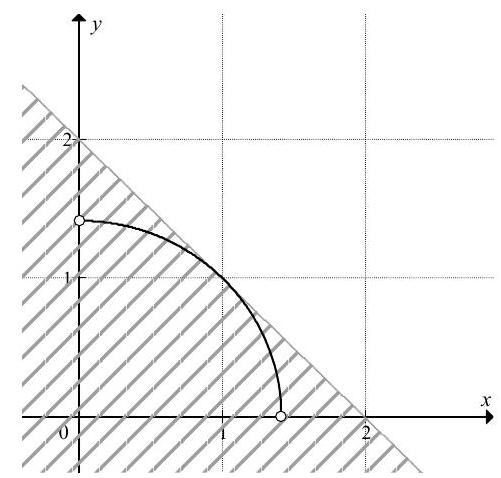
\includegraphics[max width=\textwidth, center]{2025_02_07_98a741470d4a24b1ba35g-08}

To kończy dowód.

\section*{Schemat punktowania VI sposobu rozwiązania}
Zdający otrzymuje\\
gdy zapisze, że wszystkie punkty $P=(x, y)$, których wspórrzędne spełniają równanie $x^{2}+y^{2}=2$, leżą na okręgu o środku $S=(0,0)$ i promieniu $r=\sqrt{2}$ i na tym zakończy lub dalej popełnia błędy.\\
Zdający otrzymuje\\
gdy zapisze, że wszystkie punkty $P=(x, y)$, których współrzędne spełniają równanie $x^{2}+y^{2}=2$, leżą na okręgu o środku $S=(0,0)$ i promieniu $r=\sqrt{2}$ oraz że każdy punkt okręgu leży w półpłaszczyźnie opisanej nierównością $x+y \leq 2$, ale nie stwierdzi, że krawędź tej półpłaszczyzny jest styczna do okręgu i na tym zakończy lub dalej popełnia błędy.

\section*{Zdający otrzymuje}
gdy zapisze, że wszystkie punkty $P=(x, y)$, których wspórrzędne spełniają równanie $x^{2}+y^{2}=2$, leżą na okręgu o środku $S=(0,0)$ i promieniu $r=\sqrt{2}$ oraz że każdy punkt okręgu leży w półpłaszczyźnie opisanej nierównością $x+y \leq 2$, a także stwierdzi, że prosta o równaniu $x+y=2$ jest styczna do tego okręgu.

\section*{Przykładowe rozwiązanie}
\section*{VII sposób}
Niech $x$ i $y$ będą dowolnymi dodatnimi liczbami rzeczywistymi takimi, że $x^{2}+y^{2}=2$. Stąd otrzymujemy $y^{2}=2-x^{2}$, więc $y=\sqrt{2-x^{2}}$ dla $0<x<\sqrt{2}$, gdyż $y>0$. Wówczas nierówność $x+y \leq 2$ jest równoważna nierówności

$$
\begin{aligned}
& x+\sqrt{2-x^{2}} \leq 2 \\
& \sqrt{2-x^{2}} \leq 2-x .
\end{aligned}
$$

Obie strony tej nierówności są dodatnie, gdyż $0<x<\sqrt{2}$, więc, podnosząc obie strony nierówności do kwadratu, otrzymujmy nierówność równoważną

$$
\begin{gathered}
2-x^{2} \leq 4-4 x+x^{2} \\
2 x^{2}-4 x+2 \geq 0 \\
x^{2}-2 x+1 \geq 0 \\
(x-1)^{2} \geq 0
\end{gathered}
$$

która jest prawdziwa dla każdej liczby rzeczywistej $x$. To kończy dowód.

\section*{Schemat punktowania VII sposobu rozwiązania \\
 Zdający otrzymuje}
gdy wyznaczy z równości $x^{2}+y^{2}=2$ jedną z liczb w zależności od drugiej: $y=\sqrt{2-x^{2}}$ dla $0<x<\sqrt{2}$ i na tym poprzestanie lub dalej popełnia błędy.

\section*{Zdający otrzymuje}
gdy zapisze nierówność z jedną niewiadomą, np. $x^{2}+\sqrt{2-x^{2}} \leq 2$ i na tym poprzestanie lub dalej popełnia błędy.

\section*{Zdający otrzymuje}
gdy przeprowadzi pełne rozumowanie.

\section*{Przykładowe rozwiązanie}
VIII sposób\\
Niech $x$ i $y$ będą dowolnymi dodatnimi liczbami rzeczywistymi takimi, że $x^{2}+y^{2}=2$. Stąd otrzymujemy $y=\sqrt{2-x^{2}}$ dla $0<x<\sqrt{2}$, gdyż $y>0$. Do obu stron równania $x^{2}+y^{2}=2$ dodajemy $2 x y$, otrzymując

$$
\begin{gathered}
x^{2}+y^{2}+2 x y=2+2 x y, \\
(x+y)^{2}=2+2 x y .
\end{gathered}
$$

Stąd

$$
x+y=\sqrt{2+2 x y}=\sqrt{2+2 x \sqrt{2-x^{2}}}=\sqrt{2+2 \sqrt{2 x^{2}-x^{4}}} .
$$

Rozważmy funkcję $f$ określoną dla $0<x<\sqrt{2}$ wzorem $f(x)=2+2 \sqrt{2 x^{2}-x^{4}}$.\\
Wyznaczymy największą wartość tej funkcji. Ponieważ funkcja $y=2+2 \sqrt{t}$ jest rosnąca,\\
więc funkcja $f$ osiąga największą wartość wtedy i tylko wtedy, gdy największą wartość osiąga funkcja $g$ określona dla $0<x<\sqrt{2}$ wzorem $g(x)=2 x^{2}-x^{4}$. Obliczamy pochodną tej funkcji

$$
g^{\prime}(x)=4 x-4 x^{3} \text { dla } 0<x<\sqrt{2} .
$$

Obliczamy miejsca zerowe pochodnej i badamy jej znak.\\
Ponieważ $g^{\prime}(x)=4 x(1-x)(1+x)$ oraz $4 x(1+x)>0$ dla każdego $0<x<\sqrt{2}$, więc:\\
$g^{\prime}(x)=0$ wtedy i tylko wtedy, gdy $1-x=0$, czyli $x=1$,\\
$g^{\prime}(x)>0$ wtedy i tylko wtedy, gdy $1-x>0$ i $0<x<\sqrt{2}$, czyli gdy $0<x<1$,\\
$g^{\prime}(x)<0$ wtedy i tylko wtedy, gdy $1-x<0$ i $0<x<\sqrt{2}$, czyli gdy $1<x<\sqrt{2}$.\\
Zatem w przedziale $(0,1\rangle$ funkcja $g$ jest rosnąca, w przedziale $\langle 1, \sqrt{2})$ jest malejąca, a w punkcie $x=1$ przyjmuje maksimum lokalne, które jest jednocześnie największą wartością tej funkcji.\\
Gdy $x=1$, to

$$
f(1)=2+2 \sqrt{2 \cdot 1^{2}-1^{4}}=4 .
$$

Zatem

$$
x+y \leq \sqrt{4}=2
$$

co kończy dowód.

\section*{Schemat punktowania VIII sposobu rozwiązania}
Zdający otrzymuje 1 p.\\
gdy wyznaczy sumę liczb $x$ i $y$ w zależności od jednej zmiennej, np. $x+y=\sqrt{2+2 x \sqrt{2-x^{2}}}$ dla $0<x<\sqrt{2}$ i na tym poprzestanie lub dalej popełnia błędy.\\
Zdający otrzymuje\\
gdy obliczy miejsca zerowe pochodnej i zbada jej znak, np.:\\
$g^{\prime}(x)=0$ dla $x=1, g^{\prime}(x)>0$ dla $0<x<1, g^{\prime}(x)<0$ dla $1<x<\sqrt{2}$\\
i na tym poprzestanie lub dalej popełnia błędy.\\
Zdający otrzymuje 3 p.\\
gdy przeprowadzi pełne rozumowanie.

\section*{Uwagi:}
\begin{enumerate}
  \item Jeżeli zdający jako jedyne uzasadnienie prawdziwości nierówności przywołuje „nierówność Cauchy'ego" i nie zapisuje tej nierówności ani żadnych wniosków płynących z zastosowania tej nierówności, to otrzymuje 0 punktów.
  \item Jeżeli zdający, oprócz powołania się na nazwisko Cauchy, zapisze odpowiednią nierówność Cauchy'ego, to przedstawione rozwiązanie jest oceniane tak, jak to przewiduje schemat.
  \item Jeżeli zdający nie zapisze koniecznego założenia o możliwych wartościach $x$ przy wyznaczaniu $y$ w zależności od $x$, to otrzymuje co najwyżej 2 punkty.
\end{enumerate}

Zadanie 9. (0-3)\\
V. Rozumowanie i argumentacja.

\begin{displayquote}

\begin{enumerate}
  \setcounter{enumi}{6}
  \item Planimetria. Zdający rozpoznaje figury podobne i jednokładne; wykorzystuje (także w kontekstach praktycznych) ich własności (R7.4).
\end{enumerate}
\end{displayquote}

\section*{Przykładowe rozwiązania}
\section*{I sposób}
Poprowadźmy promienie $S E$ i $S F$ okręgu o środku $S$ do punktów $E$ i $F$ styczności tego okręgu odpowiednio z przekątną $B D$ i bokiem $A B$ prostokąta. Niech $G$ będzie rzutem punktu $N$ na bok $A B$, jak na rysunku.\\
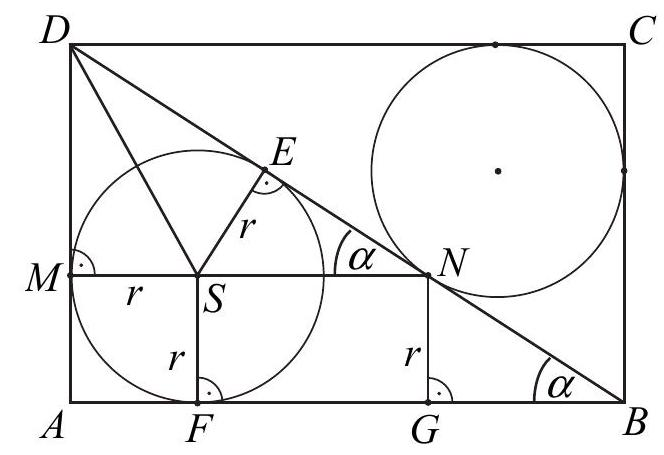
\includegraphics[max width=\textwidth, center]{2025_02_07_98a741470d4a24b1ba35g-11}

Wówczas $|S M|=|S E|=|S F|=|M A|=|N G|$ oraz $|D E|=|B N|$.\\
Trójkąty $D M S$ i $D E S$ są prostokątne, więc ztwierdzenia Pitagorasa dla tych trójkątów otrzymujemy

$$
|D M|=\sqrt{|D S|^{2}-|S M|^{2}}=\sqrt{|D S|^{2}-|S E|^{2}}=|D E| .
$$

Odcinek $M N$ jest równoległy do $A B$, więc kąty $G B N$ i $E N S$ są równe. Trójkąty $B G N$ i $N E S$ są prostokątne, więc kąty $B N G$ i $N S E$ także są równe. To z kolei wraz z równością $|S E|=|N G|$ oznacza, że trójkąty $B G N$ i $N E S$ są przystające. Zatem $|B N|=|N S|$.\\
Stąd

$$
|M N|=|M S|+|S N|=|M A|+|B N|=|M A|+|D E|=|M A|+|D M|=|A D| .
$$

To kończy dowód.

\section*{Uwaga:}
Równość odcinków $D M$ i $D E$ wynika też bezpośrednio z twierdzenia o odcinkach stycznych.

\section*{II sposób}
Poprowadźmy promienie $S E$ i $S F$ okręgu o środku $S$ do punktów $E$ i $F$ styczności tego okręgu odpowiednio z przekątną $B D$ i bokiem $A B$ prostokąta. Połączmy punkty $S$ oraz $B$, jak na rysunku.\\
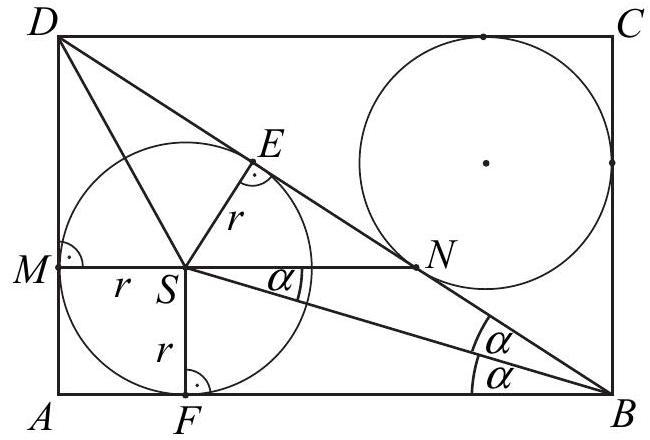
\includegraphics[max width=\textwidth, center]{2025_02_07_98a741470d4a24b1ba35g-12(1)}

Wówczas $|S M|=|S E|=|S F|=|M A|$ oraz $|D E|=|B N|$.\\
Ponieważ $|M N|=r+|S N|$ oraz $|A D|=r+|D M|$, wystarczy wykazać, że $|D M|=|S N|$.\\
Z przystawania trójkątów prostokątnych $B F S$ i $B E S$ (wspólna przeciwprostokątna i równe przyprostokątne $|S F|=|S E|$ ) otrzymujemy $|\Varangle E B S|=|\Varangle F B S|=\alpha$.\\
Odcinek $M N$ jest równoległy do $A B$, zatem kąty $F B S$ i $N S B$ są równe, jako kąty naprzemianległe, czyli kąty $N S B$ i $S B N$ także są równe. Wobec powyższego trójkąt $B S N$ jest równoramienny i $|B N|=|N S|$ oraz $|B N|=|D M|$, a stąd wynika równość $|D M|=|S N|$. To kończy dowód.

\section*{III sposób}
Poprowadźmy promienie okręgu o środku $S$ do punktów $E$ i $F$ styczności tego okręgu z bokami $B D$ i $A B$ trójkąta $D A B$. Niech $r$ oznacza promień tego okręgu, $x=|M D|, \quad y=|S N|$ i $z=|E N|$.\\
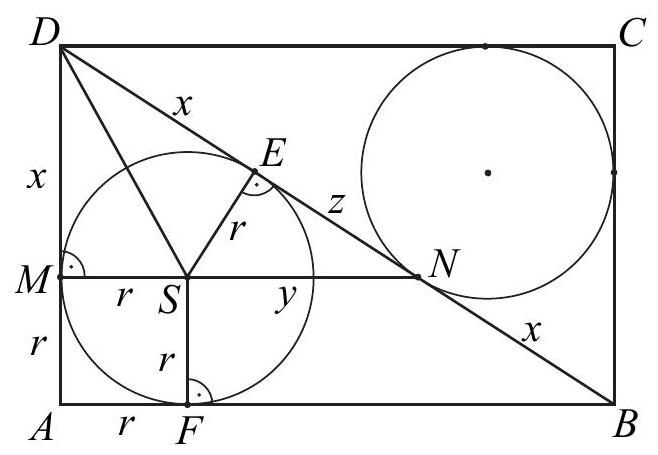
\includegraphics[max width=\textwidth, center]{2025_02_07_98a741470d4a24b1ba35g-12}

Z twierdzenia o odcinkach stycznych wynika, że $|E D|=|M D|=x$. Trójkąty $D A B$ i $C B D$ są przystające, więc $|N B|=|E D|=x$. Czworokąt $A F S M$ jest kwadratem, więc $|M A|=|A F|=r$.\\
Ponadto $|B F|=|B E|=x+z$.\\
Trójkąty $D A B$ i $D M N$ są podobne (oba są prostokątne i mają wspólny kąt ostry przy wierzchołku $D$ ). Zatem

$$
\frac{|A D|}{|D B|}=\frac{|M D|}{|D N|}, \text { czyli } \frac{r+x}{2 x+z}=\frac{x}{x+z} .
$$

Stąd

$$
\begin{gathered}
(r+x)(x+z)=(2 x+z) x, \\
r x+r z+x^{2}+x z=2 x^{2}+x z, \\
z=\frac{x^{2}-r x}{r} .
\end{gathered}
$$

Z podobieństwa trójkątów MDN i $E S N$ (oba są prostokątne i mają wspólny kąt ostry przy wierzchołku $N$ ) wynika , że

$$
\frac{|S E|}{|S N|}=\frac{|M D|}{|D N|}, \operatorname{czyli} \frac{r}{y}=\frac{x}{x+z} .
$$

Stąd i z (1) otrzymujemy

$$
y=\frac{r(x+z)}{x}=\frac{r x+r \cdot \frac{x^{2}-r x}{r}}{x}=\frac{r x+x^{2}-r x}{x}=x .
$$

To oznacza, że $|A D|=r+x=r+y=|M N|$. To kończy dowód.

\section*{Schemat punktowania}
Rozwiązanie, w którym postęp jest niewielki, ale konieczny na drodze do pełnego rozwiązania zadania

1 p.\\
Zdający

\begin{itemize}
  \item poprowadzi odcinki $S E$ i $N G$\\
albo
  \item zapisze równość $|D M|=|D E|$,\\
albo
  \item zapisze równość $|D E|=|B N|$,\\
albo
  \item zapisze równość $|S M|=|S E|=|M A|=|N G|$,\\
albo
  \item zapisze, że trójkąty $B F S$ i $B E S$ są przystające,\\
albo
  \item zapisze proporcję wynikającą z podobieństwa trójkątów $D A B$ i $D M N: \frac{|A D|}{|D B|}=\frac{|M D|}{|D N|}$,\\
albo
  \item zapisze proporcję wynikającą z podobieństwa trójkątów MDN i $E S N$ : $\frac{|S E|}{|S N|}=\frac{|M D|}{|D N|}$,\\
albo
  \item zauważy, że odcinek $B S$ jest dwusieczną kąta $A B D$,\\
albo
  \item zapisze, że trójkąt BNS jest równoramienny\\
i na tym zakończy lub dalej popełni błędy.\\
Pokonanie zasadniczych trudności zadania
\end{itemize}

\section*{Zdający}
\begin{itemize}
  \item zapisze, że trójkąty $B G N$ i $N E S$ są przystające\\
albo
  \item zapisze, że trójkąt $B S N$ jest równoramienny i $|B N|=|D M|$, albo
  \item zapisze proporcje: $\frac{r+x}{2 x+z}=\frac{x}{x+z} \mathrm{i} \frac{r}{y}=\frac{x}{x+z}$,\\
albo
  \item zauważy, że $|M N|=r+|S N|$ i $|E N|=|A B|-|A D|$,\\
albo
  \item zapisze proporcje: $\frac{r+x}{r+y+\sqrt{x^{2}-r^{2}}}=\frac{x}{r+y}$ i $\frac{r}{z}=\frac{x}{r+y}$ oraz zapisze równanie wynikające z twierdzenia Pitagorasa w jednym z trójkątów $B G N$ i $E N S$ i na tym zakończy lub dalej popełnia błędy.
\end{itemize}

Rozwiązanie pelne 3 p.

Zdający wykaże, że $|M N|=|A D|$.

\section*{Zadanie 10. (0-4)}
IV. Użycie i tworzenie strategii.\\
4. Funkcje. Zdający wykorzystuje własności funkcji liniowej i kwadratowej do interpretacji zagadnień geometrycznych, fizycznych itp. także osadzonych w kontekście praktycznym) (4.12).

\section*{Przykładowe rozwiązania}
\section*{I sposób}
Wyznaczymy najpierw współrzędne punktu przecięcia. Przyrównujemy $f(x)$ i $g(x)$, a otrzymane równanie zapisujemy w postaci

$$
(a+1) x=7
$$

Ponieważ $x>0$, więc $a+1>0$, czyli $a>-1$.\\
Zatem

$$
y=f(x)=\frac{7}{a+1}-2=\frac{5-2 a}{a+1} .
$$

Ponieważ $y>0$, a ponadto $a+1>0$, więc wynika stąd, że $5-2 a>0$, skąd otrzymujemy

$$
a<\frac{5}{2} .
$$

Łączymy oba warunki $x>0$ i $y>0$ i zapisujemy odpowiedź: punkt przecięcia wykresów funkcji ma obie współrzędne dodatnie dla $-1<a<\frac{5}{2}$.

\section*{II sposób}
Zilustrujmy w układzie współrzędnych sytuację opisaną w treści zadania.\\
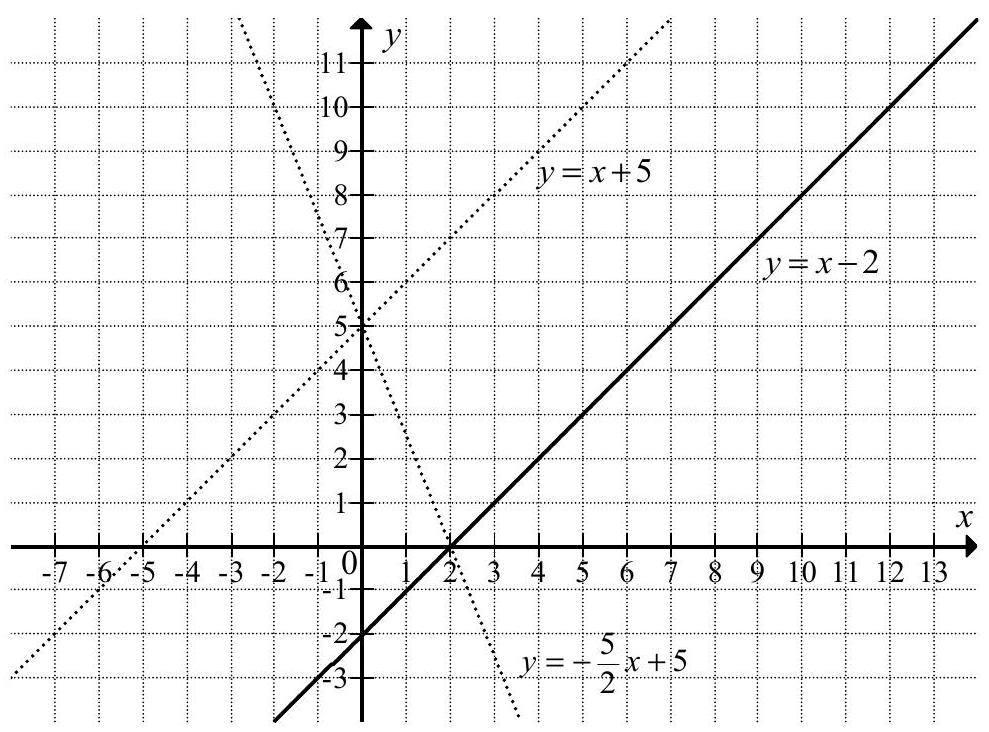
\includegraphics[max width=\textwidth, center]{2025_02_07_98a741470d4a24b1ba35g-15}

Ponieważ równanie $y=-a x+5$ opisuje pęk prostych przechodzących przez punkt o współrzędnych $(0,5)$, więc rysując proste o równaniach $y=x+5$ oraz $y=-\frac{5}{2} x+5$ (linie przerywane) otrzymujemy graniczne położenia linii prostych należących do tego pęku prosta o równaniu $y=x+5$ nie ma żadnego punktu wspólnego z prostą o równaniu $y=x-2$, natomiast prosta o równaniu $y=-\frac{5}{2} x+5$ ma jeden punkt wspólny z prostą o równaniu $y=x-2$, jest nim punkt $(2,0)$, którego współrzędne nie spełniają warunku określonego w treści tego zadania.\\
Zapisujemy odpowiedź: Punkty przecięcia wykresów funkcji mają dwie dodatnie współrzędne wtedy i tylko wtedy, gdy $-1<a<\frac{5}{2}$.

\section*{Schemat punktowania}
\section*{Rozwiązanie, w którym postęp jest niewielki, ale konieczny na drodze do pełnego rozwiązania zadania \\
 1 p.}
Zdający wyznaczy jedną ze współrzędnych punktu przecięcia w zależności od $a$ oraz zapisze:

\begin{itemize}
  \item $x=\frac{7}{a+1}$\\
albo
  \item $y=\frac{7}{a+1}-2$\\
i na tym zakończy lub dalej popełnia błędy.\\
Rozwiązanie, w którym jest istotny postęp
\end{itemize}

\section*{Zdający}
\begin{itemize}
  \item wyznaczy obie wspórrzędne punktu przecięcia w zależności od $a$ i zapisze: $x=\frac{7}{a+1}$ i $y=\frac{5-2 a}{a+1}$ dla $a \neq-1$\\
albo
  \item wyznaczy pierwszą wspórrzędną punktu przecięcia w zależności od $a: x=\frac{7}{a+1}$ i zapisze, że druga współrzędna jest dodatnia, gdy $x>2$ (o ile wynika to z przywołanej koniunkcji $x>0 \wedge x>2$ ),\\
albo
  \item zapisze, że $x>0$, gdy $a>-1$ i nie wyznaczy drugiej współrzędnej punktu przecięcia, albo
  \item sporządzi ilustrację graficzną jednej pary prostych o równaniach: $y=x-2$ i $y=x+5$ lub $y=x-2$ i $y=-\frac{5}{2} x+5$\\
i na tym zakończy lub dalej popełnia błędy.\\
Pokonanie zasadniczych trudności zadania
\end{itemize}

\section*{Zdający:}
\begin{itemize}
  \item zapisze, że dla $a>-1$ spełniona jest nierówność $x>0$ i wyznaczy drugą współrzędną\\
albo
  \item zapisze, że dla $-1<a<\frac{5}{2}$ spełniona jest nierówność $y>0$ i nie rozważy warunku $x>0$,\\
albo
  \item sporządzi ilustrację graficzną, na której znajdą się proste o równaniach:
\end{itemize}

$$
y=x+5 \quad \text { i } \quad y=-\frac{5}{2} x+5 \quad \text { i } \quad y=x-2
$$

oraz zapisze przynajmniej jedną poprawną nierówność, którą spełnia współczynnik $a$, albo

\begin{itemize}
  \item sporządzi ilustrację graficzną prostej o równaniu: $y=x-2$ i pęku prostych przechodzących przez punkt o wspórrzędnych $(0,5)$ oraz zapisze przynajmniej jedną poprawną nierówność, którą spełnia współczynnik $a$\\
i na tym zakończy lub dalej popełnia błędy.\\
Rozwiązanie pełne\\
4 p.\\
Zdający zapisze, że dla $-1<a<\frac{5}{2}$ obie współrzędne punktu przecięcia są dodatnie.
\end{itemize}

\section*{Uwagi:}
\begin{enumerate}
  \item Jeżeli zdający podstawia do równania pęku prostych współrzędne punktu ( 0,2 ), otrzymuje $a=\frac{5}{2}$ i na tym zakończy lub dalej popełni błędy, to otrzymuje 1 punkt. Jeśli dodatkowo poda, że $a<\frac{5}{2}$, to otrzymuje 2 punkty.
  \item Jeżeli zdający przedstawia rysunek, na którym jest tylko prosta o równaniu $y=x-2$, i odpowiedź $a \in\left(-1, \frac{5}{2}\right)$ bez żadnych wyjaśnień, to otrzymuje 1 punkt.
\end{enumerate}

\section*{Zadanie 11. (0-4)}
IV. Użycie i tworzenie strategii.\\
6. Trygonometria. Zdający rozwiązuje równania i nierówności trygonometryczne oraz posługuje się wykresami funkcji trygonometrycznych (R6.6, R6.4).

\section*{Przykładowe rozwiązanie}
Ponieważ $\cos ^{2} x \geq 0$ dla każdego $x$, to nierówność $\frac{2 \cos x-\sqrt{3}}{\cos ^{2} x}<0$ jest równoważna koniunkcji $2 \cos x-\sqrt{3}<0$ i $\cos x \neq 0$, czyli $\cos x<\frac{\sqrt{3}}{2}$ i $\cos x \neq 0$.\\
Zatem $x \in\left(\frac{\pi}{6}+2 k \pi, \frac{11 \pi}{6}+2 k \pi\right)$, gdzie $k$ jest liczbą całkowitą, i $x \neq \frac{\pi}{2}+m \pi$, gdzie $m$ jest liczbą całkowitą.\\
W przedziale $\langle 0,2 \pi\rangle$ rozwiązaniem tej nierówności jest każda liczba

$$
x \in\left(\frac{\pi}{6}, \frac{\pi}{2}\right) \cup\left(\frac{\pi}{2}, \frac{3 \pi}{2}\right) \cup\left(\frac{3 \pi}{2}, \frac{11 \pi}{6}\right)
$$

\section*{Uwaga:}
Nierówności $\cos x<\frac{\sqrt{3}}{2}$ i $\cos x \neq 0$ możemy rozwiązać, np. odczytując odpowiednie argumenty funkcji $f(x)=\cos x$, dla których przyjmuje ona wartości mniejsze od $\frac{\sqrt{3}}{2}$ i różne od zera.\\
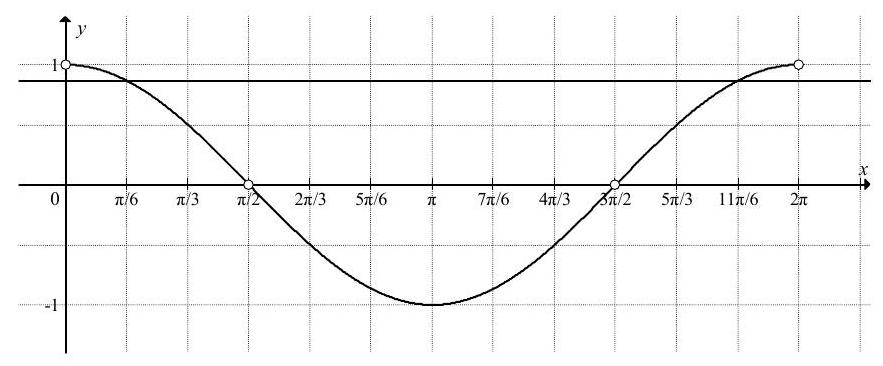
\includegraphics[max width=\textwidth, center]{2025_02_07_98a741470d4a24b1ba35g-17}

Funkcja cosinus przyjmuje w przedziale $\langle 0,2 \pi\rangle$ wartość $\frac{\sqrt{3}}{2}$ dla dwóch argumentów: $x=\frac{\pi}{6}$, $x=\frac{11 \pi}{6}$. Ma również w tym przedziale dwa miejsca zerowe: $x=\frac{\pi}{2}, x=\frac{3 \pi}{2}$.\\
Zatem zbiorem rozwiązań nierówności $\frac{2 \cos x-\sqrt{3}}{\cos ^{2} x}<0$ w przedziale $\langle 0,2 \pi\rangle$ jest suma przedziałów

$$
\left(\frac{\pi}{6}, \frac{\pi}{2}\right) \cup\left(\frac{\pi}{2}, \frac{3 \pi}{2}\right) \cup\left(\frac{3 \pi}{2}, \frac{11 \pi}{6}\right)
$$

\section*{Schemat punktowania}
Rozwiązanie, w którym postęp jest niewielki, ale konieczny na drodze do pełnego rozwiązania zadania

1 p.\\
Zdający zapisze, że nierówność $\cos ^{2} x(2 \cos x-\sqrt{3})<0$ jest równoważna koniunkcji $\cos ^{2} x \neq 0$ i $2 \cos x-\sqrt{3}<0$ i na tym zakończy lub dalej popełnia błędy.\\
Rozwiązanie, w którym jest istotny postęp\\
Zdający

\begin{itemize}
  \item zapisze, że $\cos ^{2} x \neq 0$ dla $x \neq \frac{\pi}{2}+k \pi$, gdzie $k$ jest liczbą całkowitą albo
  \item zapisze, że $\cos ^{2} x \neq 0$ dla $x \neq \frac{\pi}{2}$ i $x \neq \frac{3 \pi}{2}$ lub $\cos x \neq 0$ dla $x \neq \frac{\pi}{2}$ i $x \neq \frac{3 \pi}{2}$, albo
  \item rozwiąże nierówność $\cos x<\frac{\sqrt{3}}{2}$ w zbiorze liczb rzeczywistych:
\end{itemize}

$$
x \in\left(\frac{\pi}{6}+2 k \pi, \frac{11 \pi}{6}+2 k \pi\right), \text { gdzie } k \text { jest liczbą całkowitą, }
$$

albo

\begin{itemize}
  \item rozwiąże nierówność $\cos x<\frac{\sqrt{3}}{2} \mathrm{w}$ przedziale $\langle 0,2 \pi\rangle: x \in\left(\frac{\pi}{6}, \frac{11 \pi}{6}\right)$\\
i na tym zakończy lub dalej popełnia błędy.\\
Pokonanie zasadniczych trudności zadania 3 p.\\
Zdający zapisze, że $\cos ^{2} x \neq 0$ dla $x \neq \frac{\pi}{2}+k \pi$, gdzie $k$ jest liczbą całkowitą oraz rozwiąże nierówność $\cos x<\frac{\sqrt{3}}{2} w$ zbiorze liczb rzeczywistych: $x \in\left(\frac{\pi}{6}+2 k \pi, \frac{11 \pi}{6}+2 k \pi\right)$, gdzie $k$ jest liczbą całkowitą i na tym zakończy lub dalej popełnia błędy.
\end{itemize}

Rozwiązanie pelne 4 p.\\
Zdający rozwiąże nierówność $\cos ^{2} x(2 \cos x-\sqrt{3})<0$ w przedziale $\langle 0,2 \pi\rangle$ :

$$
x \in\left(\frac{\pi}{6}, \frac{\pi}{2}\right) \cup\left(\frac{\pi}{2}, \frac{3 \pi}{2}\right) \cup\left(\frac{3 \pi}{2}, \frac{11 \pi}{6}\right) \text { lub } x \in\left(30^{\circ}, 90^{\circ}\right) \cup\left(90^{\circ}, 270^{\circ}\right) \cup\left(270^{\circ}, 330^{\circ}\right) .
$$

\section*{Uwagi:}
\begin{enumerate}
  \item Zdający nie musi podawać rozwiązań ogólnych. Na każdym etapie rozwiązania może ograniczyć rozumowanie do przedziału $\langle 0,2 \pi\rangle$.
  \item Jeżeli zdający zapisze, że $\cos ^{2} x \neq 0$ i podaje zbiór rozwiązań nierówności w postaci $x \in\left(\frac{\pi}{6}, \frac{11 \pi}{6}\right)$ lub $x \in\left(\frac{\pi}{6}+2 k \pi, \frac{11 \pi}{6}+2 k \pi\right)$, to za całe rozwiązanie otrzymuje 3 punkty.
  \item Jeżeli zdający poda wszystkie rozwiązania równania $\cos x=0 \mathrm{w}$ przedziale $\langle 0,2 \pi\rangle$ lub wszystkie rozwiązania równania $\cos x=\frac{\sqrt{3}}{2}$ w przedziale $\langle 0,2 \pi\rangle$ i na tym zakończy lub dalej popełni błędy, to otrzymuje $\mathbf{1}$ punkt.
  \item Jeżeli zdający zapisze warunek $\cos x \neq 0$ i poda tylko $x \neq \frac{\pi}{2}+k \pi$ lub $x \neq \frac{\pi}{2}$ i na tym zakończy lub dalej popełni błędy, to otrzymuje $\mathbf{1}$ punkt.
  \item Jeżeli zdający zapisze nierówność w postaci równoważnej $\cos ^{2} x(2 \cos x-\sqrt{3})<0$, wykona podstawienie $t=\cos x$, a następnie rozwiązując nierówność $t^{2}\left(t-\frac{\sqrt{3}}{2}\right)<0$ przyjmuje, że 0 jest pierwiastkiem jednokrotnym wielomianu i konsekwentnie rozwiąże nierówność do końca, otrzymując $x \in\left(\frac{\pi}{6}, \frac{\pi}{2}\right) \cup\left(\frac{3 \pi}{2}, \frac{11 \pi}{6}\right)$, to otrzymuje 2 punkty.
\end{enumerate}

\begin{center}
\begin{tabular}{|l|l|}
\hline
 & \begin{tabular}{l}
3. Równania i nierówności. Zdający stosuje wzory Viète'a, \\
rIII. Modelowanie \\
ratematycząuje równania i nierówności liniowe i kwadratowe \\
\end{tabular} \\
 & \begin{tabular}{l}
z parametrem, rozwiązuje nierówności kwadratowe z jedną \\
niewiadomą oraz równania i nierówności z wartością bezwzględną \\
 \\
 \\
(R3.1, R3.2, 3.5, R3.9). \\
\hline
\end{tabular} \\
\hline
\end{tabular}
\end{center}

\section*{Przykładowe rozwiązanie}
Rozwiązanie zadania dzielimy na cztery etapy. W pierwszym etapie wyznaczymy wszystkie wartości parametru $m$, dla których trójmian $f$ ma dwa różne pierwiastki. W drugim, wyznaczymy te wartości parametru $m$, dla których pierwiastki trójmianu spełniają warunek $\left|x_{1}-x_{2}\right|<3$. W trzecim wyznaczamy te wartości parametru $m$, dla których pierwiastki $x_{1}, x_{2}$ są tego samego znaku. W czwartym - końcowym etapie, wyznaczymy wszystkie szukane wartości parametru $m$.

\section*{I etap}
Ponieważ trójmian $f$ ma dwa różne pierwiastki, więc wyróżnik $\Delta$ tego trójmianu jest dodatni, zatem

$$
\Delta=(2(m+1))^{2}-4 \cdot 1 \cdot(6 m+1)>0 .
$$

Nierówność $(2(m+1))^{2}-4 \cdot 1 \cdot(6 m+1)>0$ przekształcamy w sposób równoważny

$$
\begin{gathered}
4\left(m^{2}+2 m+1\right)-4 \cdot(6 m+1)>0, \\
m^{2}+2 m+1-6 m-1>0 \\
m^{2}-4 m>0, \\
m(m-4)>0
\end{gathered}
$$

Rozwiązaniem tej nierówności jest każda liczba $m \in(-\infty, 0) \cup(4,+\infty)$.

\section*{II etap}
I sposób\\
Nierówność $\left|x_{1}-x_{2}\right|<3$ można zapisać, stosując wzory na pierwiastki trójmianu kwadratowego, w postaci

$$
\begin{gathered}
\left|\frac{-b-\sqrt{\Delta}}{2 a}-\frac{-b+\sqrt{\Delta}}{2 a}\right|<3, \\
\left|\frac{-\sqrt{\Delta}}{a}\right|<3, \\
\left|\frac{-\sqrt{\Delta}}{1}\right|<3, \\
\sqrt{\Delta}<3 .
\end{gathered}
$$

Ponieważ $\Delta>0$, więc $\sqrt{\Delta}>0$. Zatem obie strony nierówności są dodatnie. Stąd $0<\Delta<9$.\\
Zatem

$$
\begin{gathered}
4\left(m^{2}+2 m+1\right)-4(6 m+1)-9<0, \\
4 m^{2}-16 m-9<0 \\
m \in\left(-\frac{1}{2}, \frac{9}{2}\right)
\end{gathered}
$$

\section*{II sposób}
Obie strony nierówności $\left|x_{1}-x_{2}\right|<3$ są dodatnie, więc podnosząc je do kwadratu, otrzymujemy nierówność równoważną

$$
\left(x_{1}-x_{2}\right)^{2}<9
$$

Tę nierówność możemy z kolei zapisać w postaci

$$
\left(x_{1}+x_{2}\right)^{2}-4 x_{1} x_{2}<9
$$

Ze wzorów Viète'a otrzymujemy nierówność z niewiadomą $m$ :

$$
\begin{gathered}
4\left(m^{2}+2 m+1\right)-4(6 m+1)-9<0 \\
m \in\left(-\frac{1}{2}, \frac{9}{2}\right)
\end{gathered}
$$

\section*{III etap}
Ponieważ pierwiastki $x_{1}, x_{2}$ są tego samego znaku, więc $x_{1} \cdot x_{2}>0$. Ze wzoru Viète'a, otrzymujemy nierówność

$$
\frac{6 m+1}{1}>0, \text { skąd } m>-\frac{1}{6}
$$

\section*{IV etap}
Wyznaczamy część wspólną zbiorów:

$$
\begin{gathered}
\left(-\frac{1}{6},+\infty\right) \\
\left(-\frac{1}{2}, \frac{9}{2}\right) \\
(-\infty, 0) \cup(4,+\infty)
\end{gathered}
$$

Ostatecznie $m \in\left(-\frac{1}{6}, 0\right) \cup\left(4, \frac{9}{2}\right)$.

\section*{Schemat punktowania}
Rozwiązanie zadania składa się z czterech etapów.

\begin{itemize}
  \item Pierwszy z nich polega na rozwiązaniu nierówności $\Delta>0$ :
\end{itemize}

$$
m \in(-\infty, 0) \cup(4,+\infty)
$$

Za poprawne rozwiązanie tego etapu zdający otrzymuje 1 punkt.

\begin{itemize}
  \item Drugi etap polega na rozwiązaniu nierówności $\left|x_{1}-x_{2}\right|<3$. Za tę część rozwiązania zdający otrzymuje 3 punkty.\\
Podział punktów za drugi etap rozwiązania:\\
1 punkt zdający otrzymuje, gdy:
  \item zapisze nierówność $\left|x_{1}-x_{2}\right|<3$ w postaci $|-\sqrt{\Delta}|<3$ lub $|\sqrt{\Delta}|<3, \operatorname{lub}\left(x_{1}-x_{2}\right)^{2}<9$ albo
  \item zapisze nierówność $\left|x_{1}-x_{2}\right|<3$ w postaci: $\left|\frac{-b-\sqrt{\Delta}}{2 a}-\frac{-b+\sqrt{\Delta}}{2 a}\right|<3 \Delta<9 \quad$ lub $\left(x_{1}+x_{2}\right)^{2}-4 x_{1} x_{2}<9$.
\end{itemize}

2 punkty zdający otrzymuje, gdy zapisze nierówność z jedną niewiadomą $m$, np.

$$
\left(-\frac{2(m+1)}{1}\right)^{2}-4 \cdot \frac{6 m+1}{1}<9
$$

3 punkty zdający otrzymuje za rozwiązanie tej nierówności: $m \in\left(-\frac{1}{2}, \frac{9}{2}\right)$.

\begin{itemize}
  \item Trzeci etap polega na ustaleniu, dla jakich $m$ pierwiastki trójmianu są tego samego znaku.\\
1 punkt zdający otrzymuje za rozwiązanie nierówności $\frac{6 m+1}{1}>0: m \in\left(-\frac{1}{6},+\infty\right)$.
  \item Czwarty etap polega na ustaleniu, dla których wartości parametru $m$ pierwiastki trójmianu spełniają wszystkie warunki zadania. Wyznaczamy część wspólną zbiorów: $\left(-\frac{1}{6},+\infty\right),\left(-\frac{1}{2}, \frac{9}{2}\right)$ i $(-\infty, 0) \cup(4,+\infty)$.
\end{itemize}

Za ten etap zdający może otrzymać $\mathbf{1}$ punkt, gdy:

\begin{itemize}
  \item poprawnie wykonał przynajmniej dwa etapy spośród I, II i III, a ponadto w każdym z etapów otrzymał niepusty i różny od zbioru liczb rzeczywistych $(R)$ zbiór rozwiązań albo
  \item poprawnie wykonał etapy I lub III i otrzymał co najmniej 2 punkty za II etap, a ponadto w każdym z etapów otrzymał niepusty i różny od zbioru liczb rzeczywistych $(R)$ zbiór rozwiązań.
\end{itemize}

\section*{Uwaga:}
Jeżeli zdający popełni błąd merytoryczny w trakcie rozwiązywania warunku $|-\sqrt{\Delta}|<3$ lub $|\sqrt{\Delta}|<3$, np. podniesie obie strony nierówności do kwadratu i otrzyma $\Delta>9$, to za II etap otrzymuje co najwyżej 1 punkt.

Zadanie 13. (0-5)

\begin{center}
\begin{tabular}{|l|l|}
\hline
\begin{tabular}{l}
IV. Użycie i tworzenie \\
strategii. \\
\end{tabular} & \begin{tabular}{l}
8. Geometria na płaszczyźnie kartezjańskiej. Zdający wyznacza \\
równanie prostej, która jest równoległa lub prostopadła do prostej \\
danej w postaci kierunkowej i przechodzi przez dany punkt, \\
oblicza wspórzędne punktu przecięcia dwóch prostych oraz \\
wyznacza współrzędne środka odcinka (8.3, 8.4, 8.5). \\
\end{tabular} \\
\hline
\end{tabular}
\end{center}

\section*{Przykładowe rozwiązanie}
Zauważamy, że jeżeli $A C$ jest przekątną czworokąta $A B C D$, wpisanego w okrąg i prosta $A C$ jest osią symetrii tego czworokąta, to ten czworokąt jest deltoidem, a trójkąty $A B C$ i $A D C$ są prostokątne. Obliczymy najpierw współrzędne wierzchołka $D$, który jest obrazem wierzchołka $B$, w symetrii osiowej względem prostej $A C$. Ponieważ prosta $B D$ jest prostopadła do prostej $A C$ i przechodzi przez punkt $B$, więc jej równanie ma postać

$$
y=-x+8
$$

Obliczamy współrzędne środka $S$ przekątnej $B D$. Ponieważ jest to punkt przecięcia prostych $A C$ i $B D$, więc wystarczy rozwiązać układ równań

$$
\left\{\begin{array}{l}
y=x+2 \\
y=-x+8
\end{array}\right.
$$

Otrzymujemy stąd $x=3$ i $y=5$. Zatem punkt $S$ ma współrzędne $S=(3,5)$. Współrzędne punktu $D$ spełniają zatem równania

$$
\frac{x_{D}+0}{2}=3 \quad \text { i } \quad \frac{y_{D}+8}{2}=5 .
$$

Stąd wynika, że $x_{D}=6$ i $y_{D}=2$, czyli $D=(6,2)$.\\
Obliczymy teraz współrzędne wierzchołka $C$. Zauważamy, że jest to punkt przecięcia prostej $A C$ i prostej $C D$, która jest prostopadła do prostej $A D$ i przechodzi przez punkt $D$.\\
Ponieważ współczynnik kierunkowy prostej $A D$ jest równy $\frac{2-32}{6-30}=\frac{5}{4}$, więc prosta $C D$ ma równanie postaci

$$
y=-\frac{4}{5}(x-6)+2 .
$$

Rozwiązujemy układ równań $\left\{\begin{array}{l}y=x+2 \\ y=-\frac{4}{5}(x-6)+2\end{array}\right.$ i otrzymujemy $\left\{\begin{array}{l}x=\frac{24}{9}=\frac{8}{3} \\ y=\frac{42}{9}=\frac{14}{3}\end{array}\right.$.\\
Zatem $C=\left(\frac{8}{3}, \frac{14}{3}\right)$.

\section*{Schemat punktowania}
Rozwiązanie zadania składa się z dwóch części. Pierwsza, to obliczenie współrzędnych punktu $D$, druga, to obliczenie współrzędnych punktu $C$. Mogą być one wykonane niezależnie od siebie, w dowolnej kolejności. Za pierwszą część rozwiązania zdający otrzymuje 2 punkty, a za drugą $\mathbf{3}$ punkty.

\section*{Schemat punktowania pierwszej części}
1 punkt przyznajemy zdającemu, który wyznaczy równanie prostej $B D: y=-x+8$ i zapisze, że punkt przecięcia prostych $A C$ i $B D$ jest środkiem odcinka $B D$ lub wykorzysta ten fakt.\\
2 punkty przyznajemy zdającemu za obliczenie współrzędnych punktu $D: D=(6,2)$.

\section*{Schemat punktowania drugiej części}
1 punkt przyznajemy zdającemu, który zapisze, że trójkąt $A D C$ jest trójkątem prostokątnym lub wykorzysta ten fakt.\\
2 punkty przyznajemy zdającemu za wyznaczenie równania prostej $C D: y=-\frac{4}{5}(x-6)+2$.\\
3 punkty przyznajemy zdającemu za obliczenie współrzędnych punktu $C$ : $C=\left(\frac{8}{3}, \frac{14}{3}\right)$.

\section*{Uwaga:}
Współrzędne punktu $C$ zdający może obliczać inaczej. Poniżej schematy przydziału 3 punktów za obliczenie współrzędnych wierzchołka $C$.

\begin{itemize}
  \item W przypadku obliczenia w pierwszej kolejności współrzędnych środka okręgu opisanego na danym czworokącie, który jest środkiem odcinka $A C$.\\
1 punkt - gdy zdający zapisze równanie $z$ jedną niewiadomą opisujące zależność $|S A|^{2}=|S B|^{2}$,\\
2 punkty - gdy zdający obliczy współrzędne punktu $S$,\\
3 punkty - gdy zdający obliczy współrzędne punktu $C$.
  \item W przypadku obliczenia współrzędnych punktu $C$, z wykorzystaniem twierdzenia Pitagorasa w trójkącie $A B C$.\\
1 punkt - gdy zdający zauważy, że trójkąt $A B C$ jest prostokątny, np. zapisze $|A C|^{2}=|A B|^{2}+|B C|^{2}$,\\
2 punkty - gdy zdający zapisze równanie z jedną niewiadomą, wynikające z twierdzenia Pitagorasa w trójkącie $A B C$,\\
3 punkty - gdy zdający obliczy wspórrzędne punktu $C$.
  \item W przypadku obliczenia współrzędnych punktu $C$, z wykorzystaniem symetralnej odcinka $A B$ i środka okręgu opisanego na czworokącie $A B C D$.\\
1 punkt - gdy zdający zapisze równanie symetralnej odcinka $A B$,\\
2 punkty - gdy zdający wyznaczy współrzędne środka okręgu przechodzącego przez punkty $A, B, C, D$,\\
3 punkty - gdy zdający obliczy współrzędne punktu $C$.
  \item W przypadku obliczenia współrzędnych punktu $C$, z wykorzystaniem kąta pomiędzy prostymi $A D$ i $A B$.\\
1 punkt - gdy zdający obliczy tangens kąta $D A B$,\\
2 punkty - gdy zdający zapisze równanie $z$ jedną niewiadomą $z$ wykorzystaniem współczynników kierunkowych prostych $B C$ i $C D$ jako tangensów odpowiednich kątów,\\
3 punkty - gdy zdający obliczy wspórrzędne punktu $C$.
  \item W przypadku obliczenia współrzędnych punktu $C$, z wykorzystaniem iloczynu skalarnego wektorów $B C$ i $B A$ (albo, po wyznaczeniu współrzędnych punktu $D$, wektorów $D A$ i $D C$ ).\\
1 punkt - gdy zdający zapisze, że wektory $B C$ i $B A$ albo $D A$ i $D C$ są prostopadłe lub wyznaczy ich współrzędne,\\
2 punkty - gdy zdający zapisze równanie $z$ jedną niewiadomą wynikające $z$ zerowania się iloczynu skalarnego wektorów,\\
3 punkty - gdy zdający obliczy współrzędne punktu $C$.
  \item W przypadku obliczenia współrzędnych punktu $C$, z wykorzystaniem równania okręgu przechodzącego przez punkty $A, B, D$.\\
1 punkt - gdy zdający zapisze układ trzech równań z trzema niewiadomymi, z którego można obliczyć współczynniki w równaniu okręgu,\\
2 punkty - gdy zdający wyznaczy równanie okręgu opisanego na trójkącie $A B D$,\\
3 punkty - gdy zdający obliczy współrzędne punktu $C$.
  \item W przypadku obliczenia współrzędnych punktu $C$, z wykorzystaniem twierdzenia cosinusów.\\
1 punkt - gdy zdający wyznaczy cosinus kąta $B A D$,\\
2 punkty - gdy zdający zastosuje twierdzenie cosinusów w trójkącie $B C D$ i zapisze równanie z jedną niewiadomą,\\
3 punkty - gdy zdający obliczy współrzędne punktu $C$.
  \item W przypadku obliczenia współrzędnych punktu $C$, z wykorzystaniem twierdzenia o wysokości w trójkącie prostokątnym $A B C$ (albo, po wyznaczeniu współrzędnych punktu $D$, w trójkącie $A C D$ ).\\
1 punkt - gdy zdający wyznaczy długości odcinków $A S$ i $B S$, lub $A S$ i $D S$, gdzie $S$ jest spodkiem wysokości trójkąta należącym do boku $A C$,\\
2 punkty - gdy zdający zastosuje twierdzenie o wysokości w trójkącie prostokątnym i zapisze równanie z jedną niewiadomą,\\
3 punkty - gdy zdający obliczy wspórrzędne punktu $C$.
\end{itemize}

\begin{center}
\begin{tabular}{|l|l|}
\hline
III. Modelowanie & \begin{tabular}{l}
10. Elementy statystyki opisowej. Teoria prawdopodobieństwa \\
i kombinatoryka. Zdajacy wykorzystuje wzory na liczbę \\
matematyczne. \\
\end{tabular} \\
\begin{tabular}{l}
permutacji, kombinacji, wariacji i wariacji z powtórzeniami do \\
zliczania obiektów w bardziej złożonych sytuacjach \\
kombinatorycznych (R10.1). \\
\end{tabular} &  \\
\hline
\end{tabular}
\end{center}

\section*{Przykładowe rozwiązania}
I sposób\\
Miejsce dla cyfry 1 wybieramy na $\binom{10}{3}$ sposobów. Na pozostałych siedmiu miejscach rozmieszczamy cyfry 2 lub 3 w dowolnym porządku na $2^{7}$ sposobów. Stosujemy regułę mnożenia i otrzymujemy

$$
\binom{10}{3} \cdot 2^{7}=120 \cdot 128=15360
$$

różnych liczb dziesięciocyfrowych, które można zapisać za pomocą cyfr $1,2,3$, w zapisie których cyfra 1 występuje w dokładnie trzy razy.

\section*{II sposób}
Rozpatrzymy trzy rozłączne przypadki, w zależności od tego, jaka cyfra została zapisana na pierwszym miejscu.

\begin{enumerate}
  \item Jeżeli na pierwszym miejscu jest cyfra 1, to miejsce dla pozostałych dwóch jedynek wybieramy na $\binom{9}{2}$ sposobów, na pozostałych siedmiu miejscach rozmieszczamy cyfrę 2 lub cyfrę 3 w dowolnym porządku na $2^{7}$ sposobów. Stosujemy regułę mnożenia i otrzymujemy
\end{enumerate}

$$
1 \cdot\binom{9}{2} \cdot 2^{7}=36 \cdot 128=4608
$$

liczb dziesięciocyfrowych, które można zapisać za pomocą cyfr 1, 2, 3, w których zapisie cyfra 1 występuje w dokładnie trzy razy, przy czym na pierwszym miejscu jest cyfra 1.\\
2. jeżeli na pierwszym miejscu jest cyfra 2, to miejsce dla trzech jedynek wybieramy na $\binom{9}{3}$\\
sposobów, na pozostałych sześciu miejscach rozmieszczamy cyfrę 2 lub cyfrę 3 w dowolnym porządku na $2^{6}$ sposobów. Stosujemy regułę mnożenia i otrzymujemy

$$
1 \cdot\binom{9}{3} \cdot 2^{6}=84 \cdot 64=5376
$$

liczb dziesięciocyfrowych, które można zapisać za pomocą cyfr 1, 2, 3, w których zapisie cyfra 1 występuje w dokładnie trzy razy, przy czym na pierwszym miejscu jest cyfra 2.\\
3. (rozumowanie analogiczne jak w p. 2.). Jeżeli na pierwszym miejscu jest cyfra 3, to miejsce dla trzech jedynek wybieramy na $\binom{9}{3}$ sposobów, na pozostałych sześciu miejscach rozmieszczamy cyfrę 2 lub cyfrę 3 w dowolnym porządku na $2^{6}$ sposobów. Stosujemy regułę mnożenia i otrzymujemy

$$
1 \cdot\binom{9}{3} \cdot 2^{6}=84 \cdot 64=5376
$$

liczb dziesięciocyfrowych, które można zapisać za pomocą cyfr $1,2,3$, w zapisie których cyfra 1 występuje w dokładnie trzy razy, przy czym na pierwszym miejscu jest cyfra 3.\\
Sumujemy liczby powstałe w każdym z trzech przypadków i otrzymujemy:

$$
4608+2 \cdot 5376=15360
$$

liczb dziesięciocyfrowych zapisanych wyłącznie za pomocą cyfr 1, 2, 3, w zapisie których cyfra 1 występuje dokładnie trzy razy.

\section*{III sposób}
Rozpatrzymy osiem rozłącznych przypadków, wyczerpujących wszystkie możliwości zapisu liczby dziesięciocyfrowej za pomocą cyfr 1, 2, 3, w których zapisie cyfra 1 występuje dokładnie trzy razy:

\begin{enumerate}
  \item w zapisie tej liczby występują 3 jedynki i 7 trójek, wtedy takich liczb jest $\frac{10!}{3!\cdot 7!}=120$,
  \item w zapisie tej liczby występują 3 jedynki, 1 dwójka i 6 trójek, wtedy takich liczb jest $\frac{10!}{3!\cdot 6!}=840$,
  \item w zapisie tej liczby występują 3 jedynki, 2 dwójki i 5 trójek, wtedy takich liczb jest $\frac{10!}{3!\cdot 2!\cdot 5!}=2520$,
  \item w zapisie tej liczby występują 3 jedynki, 3 dwójki i 4 trójki, wtedy takich liczb jest $\frac{10!}{3!\cdot 3!\cdot 4!}=4200$,
  \item w zapisie tej liczby występują 3 jedynki, 4 dwójki i 3 trójki, wtedy takich liczb jest $\frac{10!}{3!\cdot 4!\cdot 3!}=4200$,
  \item w zapisie tej liczby występują 3 jedynki, 5 dwójek i 2 trójki, wtedy takich liczb jest $\frac{10!}{3!\cdot 5!\cdot 2!}=2520$,
  \item w zapisie tej liczby występują 3 jedynki, 6 dwójek i 1 trójka, wtedy takich liczb jest $\frac{10!}{3!\cdot 6!}=840$,
  \item w zapisie tej liczby występują 3 jedynki i 7 dwójek, wtedy takich liczb jest $\frac{10!}{3!\cdot 7!}=120$.
\end{enumerate}

Sumujemy liczby otrzymane w każdym przypadku i otrzymujemy:

$$
2 \cdot(120+840+2520+4200)=2 \cdot 7680=15360
$$

różnych liczb dziesięciocyfrowych zapisanych wyłącznie za pomocą cyfr $1,2,3$, w zapisie których cyfra 1 występuje dokładnie trzy razy.

\section*{Schemat punktowania}
Rozwiązanie, w którym jest istotny postęp\\
Zdający zapisze, że:

\begin{itemize}
  \item miejsce dla cyfry 1 można wybrać na $\binom{10}{3}$ sposobów\\
albo
  \item miejsca dla cyfr 2 lub 3 można wybrać na $\binom{10}{7}$ sposobów,\\
albo
  \item cyfry 2 lub 3 można rozmieścić na $2^{7}$ sposobów,\\
albo
  \item jeżeli cyfra 1 jest na ustalonym (np. pierwszym) miejscu, to pozostałe dwie cyfry 1 można rozmieścić na $\binom{9}{2}$ sposobów,\\
albo
  \item jeżeli na ustalonym miejscu stoi jedna z cyfr 2 lub 3 , to trzy cyfry 1 można rozmieścić na $\binom{9}{3}$ sposobów,\\
albo
  \item jeżeli cyfry 1 stoją na ustalonych trzech miejscach, to jeśli w liczbie występuje $n$ cyfr 2, to cyfry 2 i 3 można rozmieścić na $\binom{7}{n}$ sposobów dla przynajmniej jednej konkretnej liczby $n$,\\
albo
  \item jest 8 rozłącznych przypadków wyczerpujących wszystkie możliwości zapisu liczby dziesięciocyfrowej za pomocą cyfr 1, 2, 3, w których zapisie cyfra 1 występuje dokładnie trzy razy\\
i na tym zakończy lub dalej popełnia błędy.\\
Pokonanie zasadniczych trudności zadania Zdający
  \item zapisze, że liczba rozpatrywanych liczb dziesięciocyfrowych jest równa np. $\binom{10}{3} \cdot 2^{7}$ albo
  \item zapisze, ile jest liczb w każdym z rozpatrywanych przypadków wyczerpujących wszystkie możliwości zapisu liczby dziesięciocyfrowej za pomocą cyfr 1, 2, 3, w których zapisie cyfra 1 występuje dokładnie trzy razy,\\
albo
  \item zapisze osiem rozłącznych przypadków wyczerpujących wszystkie możliwości zapisu liczby dziesięciocyfrowej za pomocą cyfr 1,2 , 3 , w których zapisie cyfra 1 występuje dokładnie trzy razy oraz w przynajmniej jednym przypadku zapisze liczbę takich liczb, np. $\binom{10}{3} \cdot 1$\\
i na tym zakończy lub dalej popełnia błędy.\\
Rozwiązanie pełne 3 p.\\
Zdający
  \item zapisze, że jest $\binom{10}{3} \cdot 2^{7}=15360$ liczb dziesięciocyfrowych zapisanych wyłącznie za pomocą cyfr $1,2,3$, w zapisie których cyfra 1 występuje dokładnie trzy razy\\
albo
  \item zsumuje liczby otrzymane w każdym z rozpatrywanych przypadków wyczerpujących wszystkie możliwości zapisu liczby dziesięciocyfrowej za pomocą cyfr 1, 2, 3, w których zapisie cyfra 1 występuje dokładnie trzy razy i zapisze, że jest ich 15360.
\end{itemize}

\section*{Uwagi:}
\begin{enumerate}
  \item Rozwiązanie uznajemy za pełne, jeżeli zdający zapisze liczbę rozpatrywanych liczb dziesięciocyfrowych bez użycia symbolu Newtona.
  \item Jeżeli zdający w swoim rozwiązaniu przedstawia zapisy, dla których brak bezpośredniej interpretacji kombinatorycznej i zapisom tym nie towarzyszą stosowne objaśnienia, to nie może otrzymać maksymalnej liczby punktów, przy czym za rozwiązanie, zawierające\\
jedynie zapisy pojedynczych liczb lub symboli Newtona (typu 120, 128, ( $\left.\begin{array}{c}10 \\ 7\end{array}\right)$ ), bez stosownych objaśnień, zdający otrzymuje $\mathbf{0}$ punktów, a za rozwiązanie, zawierające jedynie zapisy działań na liczbach (typu $120 \cdot 128=15360$ ), bez stosownych objaśnień zdający może otrzymać co najwyżej 1 punkt.
  \item Jeżeli zdający przedstawia rozwiązanie, w którym części zapisanych liczb lub działań na liczbach nie towarzyszą stosowne objaśnienia, to za takie rozwiązanie może otrzymać co najwyżej 2 punkty.
  \item Zdający może skorzystać ze wzoru dwumianowego Newtona i zapisać:
\end{enumerate}

$$
\binom{10}{3} \cdot\left\{\binom{7}{7}+\binom{7}{6}+\binom{7}{5}+\binom{7}{4}+\binom{7}{3}+\binom{7}{2}+\binom{7}{1}+\binom{7}{0}\right\}=\binom{10}{3} \cdot 2^{7}=120 \cdot 128=15360 .
$$

IV. Użycie i tworzenie strategii.\\
9. Stereometria. Zdający rozpoznaje w graniastosłupach i ostrosłupach kąty między ścianami, stosuje trygonometrię do obliczeń długości odcinków, miar kątów, pól powierzchni i objętości (9.4, 9.6).

\section*{Przykładowe rozwiązanie}
Strategię rozwiązania zadania można zrealizować na wiele sposobów. Każdy z nich różni się zestawem i kolejnością zastosowanych związków między odcinkami w ostrosłupie. Przyjmijmy następujące oznaczenia jak na rysunku.\\
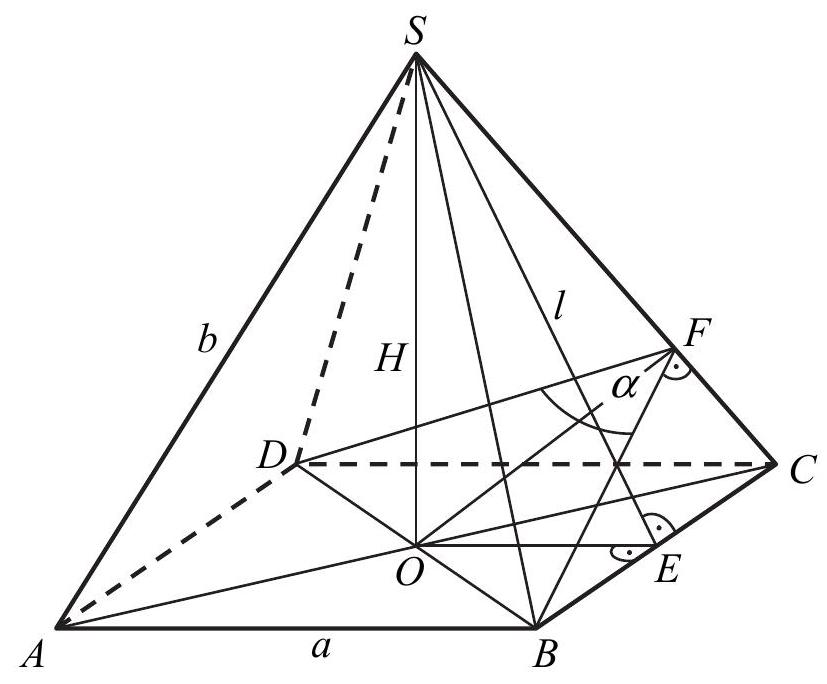
\includegraphics[max width=\textwidth, center]{2025_02_07_98a741470d4a24b1ba35g-30}

Wtedy $|O B|=\frac{a \sqrt{2}}{2},|O E|=\frac{a}{2},|\Varangle B F O|=60^{\circ}$.\\
Ponieważ trójkąt $B F O$ jest prostokątny, stąd $\frac{|B O|}{|B F|}=\sin 60^{\circ}$. Zatem

$$
|B F|=\frac{|B O|}{\sin 60^{\circ}}=\frac{\frac{a \sqrt{2}}{2}}{\frac{\sqrt{3}}{2}}=\frac{a \sqrt{2}}{2} \cdot \frac{2}{\sqrt{3}}=\frac{a \sqrt{6}}{3} .
$$

Trójkąty $S E C$ i $B F C$ są podobne, stąd $\frac{|S E|}{|S C|}=\frac{|B F|}{|B C|}$, czyli $\frac{l}{b}=\frac{\frac{a \sqrt{6}}{3}}{a}$. Zatem $l=\frac{b \sqrt{6}}{3}$.\\
Korzystamy z twierdzenia Pitagorasa w trójkątach prostokątnych EOS i BOS, skąd otrzymujemy układ równań:

$$
\left\{\begin{array}{l}
H^{2}+\left(\frac{a}{2}\right)^{2}=\left(\frac{b \sqrt{6}}{3}\right)^{2} \\
H^{2}+\left(\frac{a \sqrt{2}}{2}\right)^{2}=b^{2}
\end{array}\right.
$$

$$
\begin{aligned}
& \left\{\begin{array}{l}
25+\left(\frac{a}{2}\right)^{2}=\left(\frac{b \sqrt{6}}{3}\right)^{2} \\
25+\left(\frac{a \sqrt{2}}{2}\right)^{2}=b^{2}
\end{array}\right. \\
& \left\{\begin{array}{l}
25+\frac{a^{2}}{4}=\frac{2 b^{2}}{3} \\
25+\frac{a^{2}}{2}=b^{2}
\end{array}\right. \\
& \left\{\begin{array}{l}
300+3 a^{2}=8 b^{2} \\
50+a^{2}=2 b^{2}
\end{array}\right. \\
& \left\{\begin{array}{l}
b^{2}=75 \\
a^{2}=100
\end{array}\right. \\
& \left\{\begin{array}{l}
b=5 \sqrt{3} \\
a=10
\end{array}\right.
\end{aligned}
$$

Stąd pole $P$ podstawy $A B C D$ ostrosłupa jest równe $P=a^{2}=100$, więc objętość ostrosłupa jest równa: $V=\frac{1}{3} \cdot 100 \cdot 5=\frac{500}{3}$.

\section*{Schemat punktowania}
Rozwiązanie, w którym postęp jest niewielki, ale konieczny na drodze do pełnego rozwiązania zadania

\section*{Zdający}
\begin{itemize}
  \item zastosuje twierdzenie Pitagorasa w trójkącie $S O C$\\
albo
  \item zastosuje twierdzenie Pitagorasa w trójkącie $S O E$,\\
albo
  \item zastosuje twierdzenie cosinusów w trójkącie $B F D$,\\
albo
  \item zapisze funkcję trygonometryczną kąta ostrego w trójkącie $O B F$,\\
albo
  \item zapisze proporcję wynikającą z podobieństwa trójkątów $S E C$ i $B C F$,\\
albo
  \item zapisze proporcję wynikającą z podobieństwa trójkątów SOC i $O F C$\\
i na tym zakończy lub dalej popełnia błędy.\\
Uwaga:\\
Jeżeli zdający zapisze związki, z których można obliczyć długość krawędzi podstawy lub długość przekątnej podstawy ostrosłupa, ale pominie jedno równanie potrzebne do zakończenia obliczeń, to otrzymuje 2 punkty.
\end{itemize}

Rozwiązanie, w którym jest istotny postęp .................................................................... 3 p.\\
Zdający zapisze układ równań, z którego można obliczyć długość krawędzi podstawy lub długość przekątnej podstawy ostrosłupa i na tym zakończy lub dalej popełnia błędy.

Pokonanie zasadniczych trudności zadania\\
Zdający zapisze równanie z jedną niewiadomą oznaczającą wielkość, która pozwala obliczyć pole podstawy ostrosłupa i na tym zakończy lub dalej popełnia błędy.\\
Rozwiązanie prawie petne\\
Zdający

\begin{itemize}
  \item obliczy długość krawędzi podstawy lub długość przekątnej podstawy ostrosłupa albo
  \item obliczy długość krawędzi podstawy lub długość przekątnej podstawy ostrosłupa, popełniając błędy rachunkowe i konsekwentnie do tego obliczy objętość ostrosłupa.
\end{itemize}

\section*{Rozwiązanie pełne}
6 p.\\
Zdający obliczy objętość ostrosłupa: $V=\frac{500}{3}$.

\section*{Uwagi:}
\begin{enumerate}
  \item Jeżeli zdający rozpatruje inną bryłę, np. ostrosłup, którego podstawą nie jest kwadrat albo ostrosłup, którego ściany boczne są trójkątami równobocznymi, to otrzymuje $\mathbf{0}$ punktów.
  \item Jeżeli zdający błędnie interpretuje kąt między sąsiednimi ścianami bocznymi, ale przy korzystaniu z własności figur, w których ten kąt nie występuje, wykazuje się innymi umiejętnościami matematycznymi, to otrzymuje co najwyżej 1 punkt.
  \item Jeżeli zdający odczyta wartość $\sin \Varangle B F O=\sin 60^{\circ}$ z tablic i wykona obliczenia na przybliżeniach, to otrzymuje co najwyżej 5 punktów.
\end{enumerate}

Zadanie 16. (0-7)

\begin{center}
\begin{tabular}{l|l}
III. Modelowanie & 11. Rachunek różniczkowy. Zdający stosuje pochodne do \\
\end{tabular}
\end{center} matematyczne. rozwiązywania zagadnień optymalizacyjnych (R11.6).

\section*{Przykładowe rozwiązanie}
Niech $C=(x, y)$ będzie wierzchołkiem trapezu $A B C D$. Wówczas $C=\left(x, 2-\frac{1}{2} x^{2}\right)$, gdzie $0<x<2$. Ponieważ $|A B|=4,|C D|=2 x$, a wysokość trapezu jest równa $h=2-\frac{1}{2} x^{2}$, więc pole $P$ tego trapezu określone jest wzorem

$$
P(x)=\frac{4+2 x}{2} \cdot\left(2-\frac{1}{2} x^{2}\right)=(x+2) \cdot \frac{1}{2}\left(4-x^{2}\right)=\frac{1}{2}\left(8+4 x-2 x^{2}-x^{3}\right)=4+2 x-x^{2}-\frac{1}{2} x^{3}
$$

dla każdej liczby rzeczywistej $0<x<2$.\\
Pochodna funkcji $P(x)=4+2 x-x^{2}-\frac{1}{2} x^{3}$ jest równa $P^{\prime}(x)=2-2 x-\frac{3}{2} x^{2}$ dla $x \in(0,2)$.\\
Obliczamy miejsca zerowe pochodnej i badamy jej znak.\\
Ponieważ $P^{\prime}(x)=-\frac{3}{2}\left(x^{2}+\frac{4}{3} x-\frac{4}{3}\right)=-\frac{3}{2}\left(\left(x+\frac{2}{3}\right)^{2}-\frac{16}{9}\right)=-\frac{3}{2}\left(x-\frac{2}{3}\right)(x+2)$\\
oraz $-\frac{3}{2}(x+2)<0$ dla każdego $x \in(0,2)$, więc:\\
$P^{\prime}(x)=0$ wtedy i tylko wtedy, gdy $x=\frac{2}{3}$,\\
$P^{\prime}(x)>0$ wtedy i tylko wtedy, gdy $x-\frac{2}{3}<0$ i $x \in(0,2)$, czyli dla $x \in\left(0, \frac{2}{3}\right)$,\\
$P^{\prime}(x)<0$ wtedy i tylko wtedy, gdy $x-\frac{2}{3}>0$ i $x \in(0,2)$, czyli dla $x \in\left(\frac{2}{3}, 2\right)$.\\
Zatem w przedziale ( $\left.0, \frac{2}{3}\right\rangle$ funkcja $P$ jest rosnąca, w przedziale $\left\langle\frac{2}{3}, 2\right.$ ) jest malejąca, a w punkcie $x=\frac{2}{3}$ osiąga maksimum. Jeżeli $x=\frac{2}{3}$, to $C=\left(\frac{2}{3}, 2-\frac{1}{2} \cdot\left(\frac{2}{3}\right)^{2}\right)=\left(\frac{2}{3}, \frac{16}{9}\right)$.

Uwaga:\\
Zdający może zauważyć, że $z$ nierówności dla średniej arytmetycznej i średniej geometrycznej wynika, że dla $x \in(0,2)$ iloczyn

$$
(x+2)\left(4-x^{2}\right)=(x+2)(x+2)(2-x)=4\left(\frac{x}{2}+1\right)\left(\frac{x}{2}+1\right)(2-x)
$$

przyjmuje największą wartość równą

$$
4\left(\frac{\frac{x}{2}+1+\frac{x}{2}+1+2-x}{3}\right)^{3}=4 \cdot\left(\frac{4}{3}\right)^{3}, \text { gdy } \frac{x}{2}+1=2-x \text {, czyli dla } x=\frac{2}{3} .
$$

Takie rozumowanie zastępuje drugi etap rozwiązania.

\section*{Schemat punktowania}
Rozwiązanie zadania składa się z trzech etapów.

\begin{itemize}
  \item Pierwszy etap składa się z trzech części:\\
a) zapisanie długości podstawy $C D$ i wysokości trapezu $A B C D$ w zależności od zmiennej $x:|C D|=2 x, h=2-\frac{1}{2} x^{2}$,\\
b) zapisanie pola trapezu $A B C D$ jako funkcji zmiennej $x$ : $P(x)=\frac{4+2 x}{2} \cdot\left(2-\frac{1}{2} x^{2}\right)$ lub $P(x)=4+2 x-x^{2}-\frac{1}{2} x^{3}$,\\
c) określenie dziedziny funkcji $P:(0,2)$.
\end{itemize}

Za każdą część tego etapu zdający otrzymuje po 1 punkcie, przy czym, jeżeli zdający od razu zapisze poprawnie pole trapezu w zależności od jednej zmiennej, to otrzymuje punkt za część a) i punkt za część b).

\begin{itemize}
  \item Drugi etap składa się z trzech części:\\
a) wyznaczenie pochodnej funkcji wielomianowej $f(x)=4+2 x-x^{2}-\frac{1}{2} x^{3}$ :
\end{itemize}

$$
f^{\prime}(x)=2-2 x-\frac{3}{2} x^{2},
$$

b) obliczenie miejsc zerowych pochodnej funkcji $P: x=\frac{2}{3}$ lub pochodnej funkcji $f$ :

$$
x=-2, x=\frac{2}{3},
$$

c) zbadanie znaku pochodnej funkcji $P$ i uzasadnienie, że dla $x=\frac{2}{3}$ funkcja $P$ osiąga wartość największą.

\section*{Uwaga:}
Znak pochodnej zdający może zaznaczyć w inny sposób, np. na rysunku szkicując krzywą zbliżoną do wykresu pochodnej.

\begin{itemize}
  \item Trzeci etap.
\end{itemize}

Obliczenie współrzędnych wierzchołka $C$ tego z rozpatrywanych trapezów, którego pole jest największe:

$$
C=\left(\frac{2}{3}, \frac{16}{9}\right) .
$$

Za poprawne rozwiązanie tego etapu zdający otrzymuje 1 punkt.

\section*{Uwagi:}
\begin{enumerate}
  \item Jeżeli zdający zapisze pole trapezu $P$ z pominięciem czynnika $\frac{1}{2}$, we wzorze na pole trapezu, lub z błędem rachunkowym, to może otrzymać co najwyżej 6 punktów.
  \item Jeżeli zdający zapisze pole trapezu $P$ z błędem rzeczowym, innym niż opisany w uwadze 1., to może otrzymać co najwyżej 1 punkt za całe rozwiązanie, a jeżeli dodatkowo wyznaczy dziedzinę funkcji $P$, to może otrzymać co najwyżej 2 punkty za całe rozwiązanie.
  \item Jeżeli zdający obliczy pochodną funkcji $P$ z błędem rachunkowym i otrzyma jako $P^{\prime}$ funkcję liniową albo funkcję kwadratową o ujemnym wyróżniku $\Delta$ lub o wyróżniku $\Delta$ równym 0 , to może otrzymać punkty jedynie za I etap rozwiązania.
  \item Jeżeli zdający poprawnie wyznaczy pochodną $P^{\prime}$ i współrzędne punktu $C$, ale nie poda poprawnego uzasadnienia, dotyczącego istnienia największej wartości funkcji $P$ dla obliczonych współrzędnych, to może otrzymać co najwyżej 5 punktów.
\end{enumerate}


\end{document}